\documentclass{report}
\usepackage{graphicx}
\usepackage{textgreek}
\usepackage{fixltx2e}
\graphicspath{{Figures/}}


\begin{document}
	\title{Catenary}
	\author{Andrea Turchetto}

	\maketitle
		
	\begin{abstract}
		This document presents the equations used for the solution of the elastic catenary.
	\end{abstract}
	
	\tableofcontents
	\listoffigures
	
	\chapter{Catenary}	
	
	\section{Introduction}
	A catenary is the curve that an idealized hanging chain or cable assumes under its own weight when supported only at its ends.
	Figure \ref{CatenaryFigure} shows an example of catenary curve.
	
	\begin{figure}[h]
		\centering
		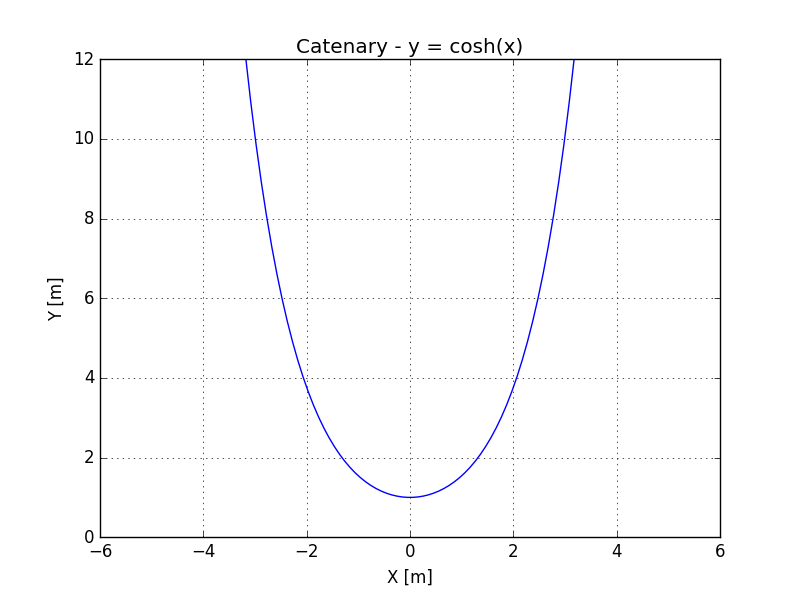
\includegraphics[width=3.0in]{Catenary.png}
		\caption{Catenary - inelastic}
		\label{CatenaryFigure}		
	\end{figure}
	
	\section{Equations - inelastic}
	The catenary equation for an inelastic cable is as follow:
	
	\begin{equation}
	\label{eq1.1}
	\frac{d}{d\theta}T(\theta) = T(\theta)\cdot\tan(\theta)
	\end{equation}
	\begin{equation}
	\label{eq1.2}
	\frac{T(\theta)}{\cos(\theta)}\cdot\frac{d}{ds}\theta = w
	\end{equation}
	
	where:
	\textit{ds} is the an element of unit length on the cable, \textit{w} is the weight per unit length of the cable, \textit{T} is the local tension, 
	\texttheta is the angle between the local tension and the horizontal and 
	T\textsubscript{H} is the horizontal tension that is constant along the cable and is given by:
	
	\begin{equation}
	\label{eq1.3}
	T_H = T\cdot\cos(\theta) = costant
	\end{equation}
	
	Combining \ref{eq1.1} with \ref{eq1.2} and \ref{eq1.3} we have:
	\begin{equation}
	\label{eq1.4}
	\frac{T_H}{\cos(\theta)^2}\cdot\frac{d}{ds}\theta = w
	\end{equation}
	
	\section{Catenary Equation - Elastic}
	This section presents the catenary equation for elastic cable (line). In this case the length of the line varies according to the applied tension at its ends.
	Assuming that as the line stretches its total weight is preserved and that the strain is linear (linear stiffness):
	\begin{equation}
	\label{eq1.5}
	w_0 = w\left(1+\frac{T}{EA}\right) = w\left(1+\frac{T_H}{EA\cdot\cos(\theta)}\right)
	\end{equation}
	where \textit{w} is the weight per unit length of the line, \textit{E} is the Young Modulus of the line and \textit{A} is the sectional area of the line.
	The solution equations for the elastic catenary are:
	\begin{equation}
	\label{eq1.6}
	s(\theta) = c\cdot\tan(\theta)+\frac{1}{2}\cdot\frac{T_H}{EA}\cdot c\cdot\tan(\theta)\cdot\sec(\theta)+\frac{1}{2}\cdot\frac{T_H}{EA}\cdot c\cdot\ln\left(\sec(\theta)+\tan(\theta)\right)
	\end{equation}
	\begin{equation}
	\label{eq1.7}
	x(\theta) = c\cdot\ln\left(\sec(\theta)+\tan(\theta)\right)+c\cdot\tan(\theta)\cdot\frac{T_H}{EA}
	\end{equation}
	\begin{equation}
	\label{eq1.8}
	y(\theta) = c\cdot\sec(\theta)\cdot\left(1+\frac{1}{2}\cdot\frac{T_H}{EA}\cdot\sec(\theta)\right)
	\end{equation}
	where
	\begin{equation}
	\label{eq1.9}
	c = \frac{T_H}{w_0}
	\end{equation}
	It is good practice to check whether the distance between the fairlead (maximum \texttheta) and the lowest (minimum) point of the catenary (vertical tension is null and \texttheta = 0) is equal to the vertical distance between the fairlead and the seabed (\textit{h}):
	\begin{equation}
	\label{eq1.10}
	h = \Delta y =  c\cdot\sec(\theta_Max)\cdot\left(1+\frac{1}{2}\cdot\frac{T_H}{EA}\cdot\sec(\theta_Max)\right) - c\cdot\sec(0)\cdot\left(1+\frac{1}{2}\cdot\frac{T_H}{EA}\cdot\sec(0)\right)
	\end{equation}
	
	
	\chapter{Conclusions}
	
\end{document}